\section{Analysis}

\subsection{Principal Component analysis and t-SNE}
To gain additional insight on how the different word embedding capture important information about each of the language classes we thought it would be interesting to try and visualize the embeddings using two different techniques for dimensionality reduction.

No matter which way we choose to extract the feature vectors they belong to a high dimensional feature space and in order to do visualization we need to project the feature vectors down to 2d space.

To do this we have implemented two different methods: Principal Component Analysis (PCA) which we will compare with T-distributed Stochastic Neighbor Embedding (t-SNE).
Here we will begin with a brief explanation of the two techniques and proceed with an analysis of the results.

\paragraph{Principal Component Analysis}

The first step is to calculate the covariance matrix of the data set.
The components of the covariance matrix is given by

\begin{align}
K_{X_i,X_j} = E[(X_i - \mu_i )(X_j -  \mu_j)]
\end{align}

where $X_{i}$ is the $i$th component of the feature vector and $\mu_{i}$ is the mean of that component.

In matrix form we can thus write the covariance matrix as
\begin{align}
K(\mathbf{x},\mathbf{z}) =
\begin{bmatrix}
    \text{cov}(x_1,z_1) &  \dots  & \text{cov}(x_1,z_n) \\
    \vdots & \ddots     & \vdots \\
    \text{cov}(x_n,z_1) & \dots  & \text{cov}(x_n,z_n) \\
\end{bmatrix}
\end{align}
The next step is to calculate the eigenvectors and eigenvalues of the covariance matrix by solving the eigenvalue equation.
\begin{align}
\det (K v-\lambda v) = 0
\end{align}
The eigenvalues are the variances along the direction of the eigenvectors or "Principal Components". To project our data set onto 2D space we select the two eigenvectors largest associated eigenvalue and project our data set onto this subspace.

In Figure \ref{pca} we see the result of running the PCA algorithm on the wikipedia data set where we have used character level bigrams as features as well as the cbow and skipgram models from FastTest.


\begin{figure}[h!]
    \centering
    \begin{subfigure}[b]{0.47\textwidth}
        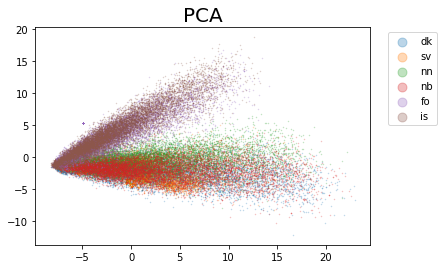
\includegraphics[width=\textwidth]{figs/pcachar2}
        \caption{Character bigram}
    \end{subfigure}
    ~
    \begin{subfigure}[b]{0.47\textwidth}
        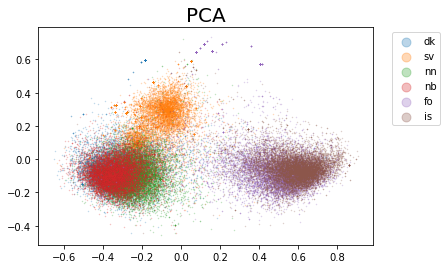
\includegraphics[width=\textwidth]{figs/pcacbow1}
        \caption{Fasttext cbow}
    \end{subfigure}
    ~
    \begin{subfigure}[b]{0.47\textwidth}
        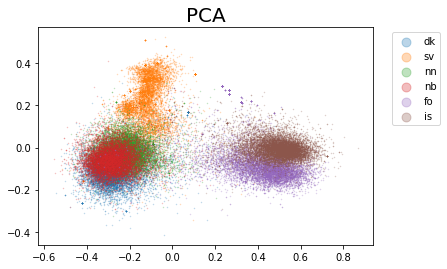
\includegraphics[width=\textwidth]{figs/pcaskipgram1}
        \caption{Fasttext skipgram}
    \end{subfigure}
    \caption{Dimensionality reduction using PCA}
    \label{pca}
\end{figure}

In the figure for encoding with character level bi-grams the PCA algorithm resulted in two elongated clusters. Without giving any prior information about the language of each sentences the PCA is apparently able to discriminate between Danish, Swedish, Nynorsk and Bokmål on one side and Faroese and Icelandic on the other since the majority of the sentences in each language belong to either of these two clusters. With the FastText implementations we observe three clusters.s

For both cbow and skipgram we see a distinct cluster of Sweedish sentences. When comparing the two FastText models we see that the t-SNE algorithm with skipgrams seems to be able to separate the Faroese and Icelandic data points to a high d ecree compared with the cbow model. Also for the cluster identified with the sentences with Danish, Bokmål and Nynorsk the skipgram models seem seem to give a better separation, however to a lesser degree than with the two former languages.

\paragraph{t-SNE}

The T-distributed Stochastic Neighbor Embedding method was first proposed in 2008 in the paper "Visualizing Data using t-SNE"\cite{tsne}.

In the paper the authors explain the theory behind the algorithm which we  will make a brief summary of here.

Suppose you pick a data point $x_i$, then the probability of picking another data point $x_j$ as a neighbor to $x_i$ is given by
\begin{align}
p_{ji}= \frac{\exp (|| x_i - x_j ||^2/2\sigma_i^2 )}{\sum_{k\neq i} \exp (|| x_i - x_k ||^2/2\sigma_i^2 )}
\end{align}

Now having this probability distribution the goal is to find the low-dimensional mapping of the data points $x_i$ which we denote $y_i$ follow a similar distribution. To solve what is referred to as the "crowding problem" the t-SNE algorithm uses the Student t-distribution which is given by
\begin{align}
q_{ij}= \frac{ (1+|| y_i - y_j ||^2 )^{-1}}{\sum_{k\neq l} (1+|| y_k - y_l ||^2 )^{-1}}
\end{align}
Now finally for optimizing this distribution is done by using gradient decent on the Kullback-Leibler divergence which is given by
\begin{align}
\frac{\delta C}{\delta y_i}= 4 \sum_j (p_{ij} - q_{ij})(y_i-y_j)(1+ || y_i - y_j ||^2  )^{-1}
\end{align}
The result from running the t-SNE algorithm on the Wikipedia data set can be seen in Figure \ref{tsne}. As was the case with the PCA algorithm it appears that the encoding with FastText seem to capture the most relevant information to discriminate between the languages, especially the skip-gram mode seems to do a good job in capturing relevant information.

\begin{figure}[h!]
    \centering
    \begin{subfigure}[b]{0.47\textwidth}
        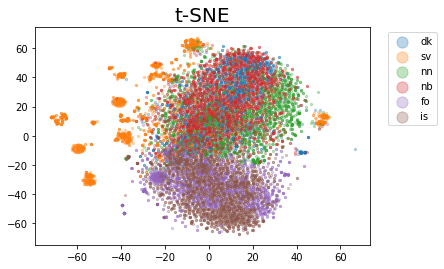
\includegraphics[width=\textwidth]{figs/tsnechar2}
        \caption{Character bi-gram}
    \end{subfigure}
    ~
    \begin{subfigure}[b]{0.47\textwidth}
        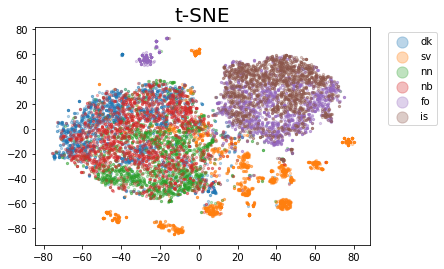
\includegraphics[width=\textwidth]{figs/tsnecbow1}
        \caption{FastText CBOW}
    \end{subfigure}
    ~
    \begin{subfigure}[b]{0.47\textwidth}
        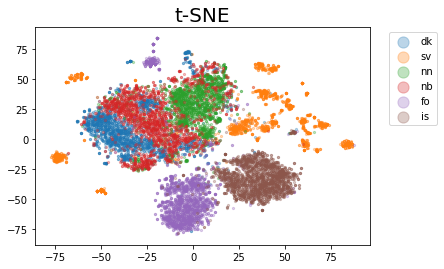
\includegraphics[width=\textwidth]{figs/tsneskipgram1}
        \caption{FastText skip-gram}
    \end{subfigure}
    \caption{Dimensionality reduction using t-SNE}
    \label{tsne}
\end{figure}


Here we recover some interesting information about the similarity of the languages. The data points in Bokmål lies in between those in Danish and Nynorsk while Icelandic and Faroese have their own two clusters which are separated from the three former languages. 

This is in good agreement with what we already know about the languages. Interestingly the Swedish data points and quite scattered and the t-SNE is not able to make a coherent Swedish cluster.

This does not however mean that the Swedish datapoint are not close in the original space. Some care is needed when interpreting the plot since t-SNE groups together data points such that neighboring points in the input space will tend to be neighbors in the low dimensional space.

If points are separated in input space, t-SNE would like to separate them in the low dimensional space however it does not care how far they are separated. So clusters that are far away in the low dimensional space are not necessarily far away in the input space.

\subsection{Discussion}
We used the dimensionality reduction techniques PCA and t-SNE to make visualizations of feature vectors obtained by making a one-hot encoding with character bi-grams and with the two modes from FastText.

These unsupervised techniques was able to separate the sentences from Wikipedia into different clusters.
Without any prior knowledge about the actual language of each sentence these techniques indicated that the six languages can be divided into three main language categories: (1) Danish Nynorsk Bokmål (2) Faroese Icelandic and (3) Swedish.


Generally the supervised models had the largest errors when discriminating between languages belonging to either of the language groups mentioned above.

For the "classical" models we saw that Logistic Regression and support vector machines achieved better performance than Knn and Naive Bayes, where the latter performed the worst. This was true in all cases irrespective of the method of feature extraction.

Additionally we saw that when we used feature vectors from the FastText skip-gram model the classification models achieved better results than when using either FastText CBOW or character n-grams.

Generally we saw that increasing the number of data points lead to better performance. When comparing the CNN with the "classical" models however the CNN performed better than any of the other models even when trained on less data points. In this way it seems that the CNN is able to learn more from less data when compared to the other models.
